\section{Описание практической части}
\label{sec:Chapter4} \index{Chapter4}

% Если в рамках работы писался какой-то код, здесь должно быть его
% описание: выбранный язык и библиотеки и мотивы выбора, архитектура,
% схема функционирования, теоретическая сложность алгоритма, характеристики
% функционирования (скорость/память).

\subsection{Построение шаблона}
Для выполнения поставленных задач, прежде всего требуется оценить насколько часто конструкции, содержащие в себе ленивые вычисления, могут встречаться в коде. Для этого необходимо выбрать шаблон, по которому можно определить ленивые вычисления, требуемый для поиска потенциальных кандидатов для векторизации. Следует также определить стартовую точку для построения этого шаблона и реализовать отбор среди кандидатов на предмет наличия тех или иных зависимостей.

Определимся каким условиям должен удовлетворять шаблон, требуемый для задачи. 

\textit{Первым условием} является поиск стартовой точки, с которой будет начинаться построение шаблона. \textit{Стартовая точка} - определение начала участка кода, который будет подвергаться векторизации. В работе за стартовые точки векторизации были приняты операции чтения из памяти, поскольку в последующем они будут объединяться в одну операцию. Так как целью работы является векторизация ленивых вычислений, то все инструкции чтения из памяти не подходят. Необходимо найти такие инструкции обращения в память, которые находятся внутри условия if-else конструкции. Пример представлен на рисунке \todo[number].

\begin{figure}[!htb]
    \centering
    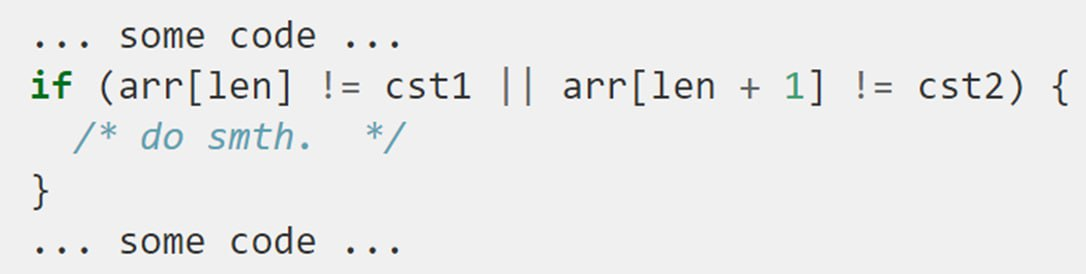
\includegraphics[scale=0.7]{lazyeval.jpg}
    \caption{Пример шаблона ленивых вычислений, требуемый для поиска и векторизации\todo[добавить 2 и более условия - переделать рисунок]}
\end{figure}

Соотвественно, \textit{вторым условием} для построения шаблона является наличие инструкций ветвления. Поскольку оптимизация проводится на уровне IR, то непосредственный интерес представляют базовые блоки, конечными инструкциями которых являются условные переходы. Ввиду того, что для векторизации необходимо два или более обращений в память и каждое из условий if-else конструкции представлено отдельным базовым блоком из-за специфики самого IR и определения базового блока, то требуется найти цепочку из базовых блоков, связанных между собой условными переходами и удовлетворяющих условию выше.

Приступая к \textit{третьему условию}, необходимо напомнить, что базовые блоки соединены между собой дугами (подробнее в \todo[глава]). Базовые блоки из набранной цепочки имеют две выходящих дуги, так как оканчиваются на условные переходы. Одна из дуг каждого базового блока должна быть входящей дугой для следующего, а вторая дуга должна соединять с одним и тем же базовым блоком, который по сути является продолжением потока управления в случае \textit{выполнения (оператор ИЛИ)} или же \textit{невыполения (оператор И)} условия. Пример подходящего шаблона представлен на рис. \todo[рисунок]

% Введем понятие шага векторизации.

% Шаг векторизации - это константа, равная размеру типа, или же в случае обращения по индексу массива, равная 1.
% \todo[убрать оставить только размер типа]

Самой сложной частью является определение \textit{соседства} операций чтения из памяти. Под \textit{соседством} в данном случае подразумевается, что данные в памяти лежат рядом друг с другом. В случае двух соседних элеметов массива это гарантируется линейной моделью памяти, упоминаемой в пункте 3.3 в работе (\todo[работа]). В коде же данное свойство представлено несколькими обращениями в память, отличающимися лишь смещением на константу, равную размеру типа. Пример такой ситуации представлен так же на рис. \todo[номер]. 

Таким образом, \textit{четвертым условием} является поиск таких обращений в память, которые являются \textit{соседними}. Поскольку промежуточное представление использует SSA-форму (рассмотрено в главе \todo[глава]), то задача поиска \textit{соседних} операций загрузки из памяти представляет собою задачу построения PSF-формы (подробнее в главе \todo[глава]). В SSA-форме каждый объект имеет ровно одно \textit{определение}, поэтому на момент сравнения двух обращений в память вовсе непонятно являются ли они \textit{соседними}, так как имеют разные определения. Помимо этого, в инструкции загрузки из памяти зачастую теряется информация о смещении (относительно начала указателя). 

Чтобы решить данную проблему, введем понятие терма. \textit{Терм} - это операнд (\textit{использование}) или результат операции (\textit{определение}), не являющийся константой, который удовлетворяет одному из следующих условий:

\begin{itemize}
    \item Базовый блок, в котором находится \textit{терм}, доминирует любой базовый блок из найденной цепочки
    \item Инструкция, содержащая \textit{терм}, не является присваиванием в SSA, то есть не удовлетворяет виду (\todo[ссылка на формулу])
\end{itemize}

Теперь можно провести следующий анализ. Для всех операций чтения из памяти, представленных в найденной цепочке и содержащихся внутри условий if-else конструкции, строится дерево, состоящее из \textit{термов} данной инструкции. Построение дерева происходит рекурсивно. Берется инструкция, для операндов которой находятся их \textit{определения}, далее в этих \textit{определениях} снова берутся операнды, для которых так же находятся \textit{определения} и так пока не будут найдены все термы. Если же некоторые операнды оказываются константой, то они суммируются и сохраняются для последующего анализа. Теперь можно утверждать следующее:

\begin{itemize}
    \item Если деревья \textit{термов} всех операций чтения из памяти являются одинаковыми, то есть все \textit{термы} совпадают друг с другом, и посчитанные суммы констант для каждого дерева в отдельности образуют числовую последовательность с шагом равным размеру типа обращения в память, то такие обращения можно считать \textit{соседними}.
\end{itemize}

Рисунок \todo[рисунок дерева и примера гимпла иллюстрирующий поиск вверх] иллюстрирует работу вышеописанного алгоритма на примере GIMPLE IR (а) и последующее построение дерева (б).

\todo[чекнуть код че я там еще делал, заменить на курсив соседние и остальную хрень]

После завершения построения шаблона было определено его количество встречаемости в коде. Для сбора информации использовались задачи из пакета CPUBench и SPEC CPU 2017. 8088 подобных шаблонов было обнаружено в наборе задач CPUBench и 5680 в SPEC CPU 2017.

\subsection{Отбор кандидатов}
сайд эффекты
из юз аутсайд
еще че то
\subsection{Версионирование кода}
сплит бб 
условие на одну страницу 4095 и создание версионного бб
картинка результата
может про ренейм мапу (необязательно)

\subsection{Ограничения предлагаемого подхода}

\newpage
